\documentclass[tikz]{standalone}

% Font
\usepackage{mathpazo}
\usepackage{libertine}
\renewcommand*\sfdefault{phv}

\large

% Color
\usepackage{xcolor}
\definecolor{f1}{HTML}{F39019}
\definecolor{b1}{HTML}{DE6A10}
\definecolor{f2}{HTML}{51A7F9}
\definecolor{b2}{HTML}{0365C0}
\definecolor{f3}{HTML}{70BF41}
\definecolor{b3}{HTML}{00882B}

% tikz
\usepackage{tikz}
\tikzstyle{every node}=[font=\sffamily]
\usetikzlibrary{shapes,arrows,positioning,calc,decorations.markings,backgrounds}
\tikzstyle{c1} = [thick,draw=b1,fill=f1]
\tikzstyle{c2} = [thick,draw=b2,fill=f2]
\tikzstyle{c3} = [thick,draw=b3,fill=f3]
\tikzstyle{cg} = [thick,draw=gray!50,fill=gray!30]
\tikzstyle{rect} = [rectangle, minimum height=1cm]
\tikzstyle{roundrect} = [rect, rounded corners=.2cm]
\tikzstyle{io} = [trapezium, trapezium left angle=70, trapezium right angle=110]
\tikzstyle{arrow} = [thick,->,>=stealth]

\tikzstyle{tag} = [minimum height=.7cm]

\begin{document}
	
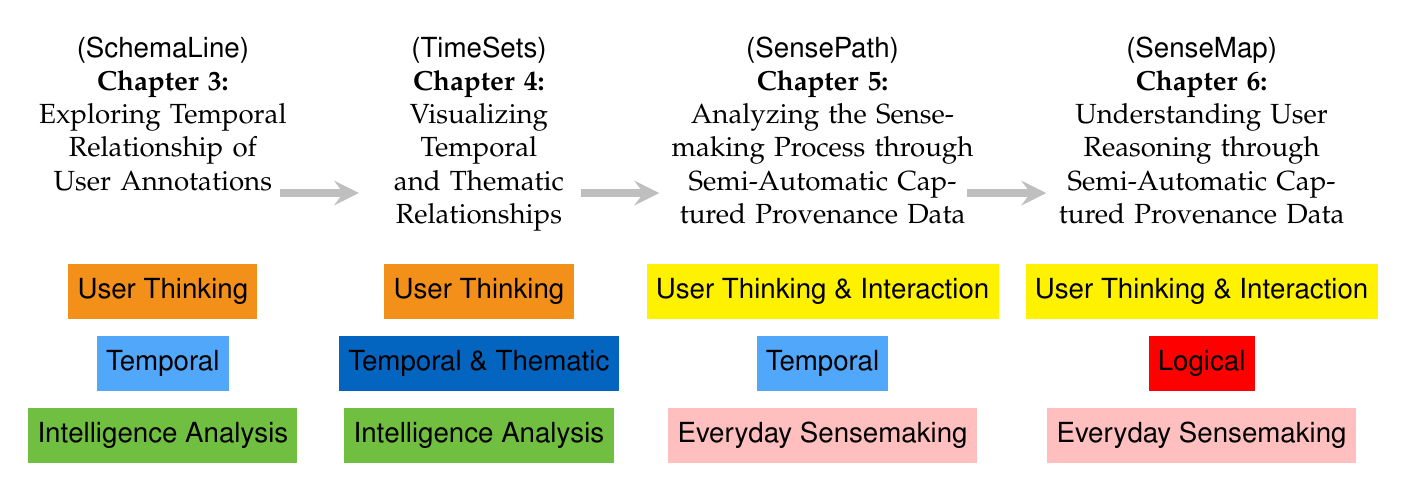
\begin{tikzpicture}[node distance=1cm]
\node (b1) [minimum width=3.2cm, minimum height=4.2cm] {};
\node (w1) [text width=3.2cm, align=center, below=0 of b1.north west, anchor=north west] {(SchemaLine)\\ \rmfamily \textbf{Chapter 3:} \\Exploring Temporal Relationship of User Annotations};
\node (data1) [tag, fill=f1, below=3 of w1.north] {User Thinking};
\node (dim1) [tag, fill=f2, below=0.2 of data1] {Temporal};
\node (dom1) [tag, fill=f3, below=0.2 of dim1] {Intelligence Analysis};

\node (b2) [minimum width=2.8cm, minimum height=4.2cm, right=of b1] {};
\node (w2) [text width=2.8cm, align=center, below=0 of b2.north west, anchor=north west] {(TimeSets)\\ \rmfamily \textbf{Chapter 4:} \\Visualizing Temporal and Thematic Relationships};
\node (data2) [tag, fill=f1, below=3 of w2.north] {User Thinking};
\node (dim2) [tag, fill=b2, below=0.2 of data2] {Temporal \& Thematic};
\node (dom2) [tag, fill=f3, below=0.2 of dim2] {Intelligence Analysis};

\node (b3) [minimum width=3.9cm, minimum height=4.2cm, right=of b2] {};
\node (w3) [text width=3.9cm, align=center, below=0 of b3.north west, anchor=north west] {(SensePath)\\ \rmfamily \textbf{Chapter 5:} \\Analyzing the Sensemaking Process through Semi-Automatic Captured Provenance Data};
\node (data3) [tag, fill=yellow, below=3 of w3.north] {User Thinking \& Interaction};
\node (dim3) [tag, fill=f2, below=0.2 of data3] {Temporal};
\node (dom3) [tag, fill=pink, below=0.2 of dim3] {Everyday Sensemaking};

\node (b4) [minimum width=3.7cm, minimum height=4.2cm, right=of b3] {};
\node (w4) [text width=3.7cm, align=center, below=0 of b4.north west, anchor=north west] {(SenseMap)\\ \rmfamily \textbf{Chapter 6:} \\Understanding User Reasoning through Semi-Automatic Captured Provenance Data};
\node (data4) [tag, fill=yellow, below=3 of w4.north] {User Thinking \& Interaction};
\node (dim4) [tag, fill=red, below=0.2 of data4] {Logical};
\node (dom4) [tag, fill=pink, below=0.2 of dim4] {Everyday Sensemaking};

\draw [arrow, cg, line width=.1cm] (b1) -- (b2);
\draw [arrow, cg, line width=.1cm] (b2) -- (b3);
\draw [arrow, cg, line width=.1cm] (b3) -- (b4);

\end{tikzpicture}

	
\end{document}